\documentclass[12pt,a4paper]{article}
\usepackage{solutions}
\usepackage{float}

\title{Листочек 1. Равномерно асимптотический.\\Математический анализ. 1 курс.\\Решения.}
\author{Глеб Минаев @ 102 (20.Б02-мкн)}
% \date{}

\DeclareMathOperator{\sign}{sign}
\renewcommand{\Re}{\qopname\relax o{Re}}
\renewcommand{\Im}{\qopname\relax o{Im}}

\begin{document}
    \maketitle
    \section*{Базовые задачи}

    \begin{enumproblem}
        TBP
        % Для начала рассмотрим функцию $f: \RR \to \RR$, определённую по правилу
        % \[
        %     f(x) := \begin{cases}
        %         e^{-\frac{1}{x^2} - \frac{1}{(x-1)^2}}& \text{если $x \in (0; 1)$}\\
        %         0& \text{иначе}
        %     \end{cases}
        % \]
        % Заметим, что $f \in C^\infty(\RR)$. Действительно, покажем, что для каждого $n$ есть многочлены $P_n$ и $Q_n$, что
        % \[
        %     f^{(n)}(x) = \begin{cases}
        %         \frac{P_n(x)}{Q_n(x)} e^{-\frac{1}{x^2} - \frac{1}{(x-1)^2}}& \text{если $x \in (0; 1)$}\\
        %         0& \text{иначе}
        %     \end{cases}
        % \]
        % Действительно, если утверждение верно для $n$, то заметим, что для $x \in (0; 1)$
        % \begin{align*}
        %     f^{(n+1)}(x)
        %     &= \Biggl(\frac{P_n(x)}{Q_n(x)} e^{-\frac{1}{x^2} - \frac{1}{(x-1)^2}}\Biggr)'\\
        %     &= \left(\frac{P_n(x)}{Q_n(x)}\right)' e^{-\frac{1}{x^2} - \frac{1}{(x-1)^2}} + \frac{P_n(x)}{Q_n(x)} \left(e^{-\frac{1}{x^2} - \frac{1}{(x-1)^2}}\right)'\\
        %     &= \frac{P'_n(x)Q_n(x) - P_n(x)Q'_n(x)}{Q_n(x)^2} \cdot e^{-\frac{1}{x^2} - \frac{1}{(x-1)^2}}
        %         + \frac{P_n(x)}{Q_n(x)} \left(\frac{2}{x^3}+\frac{2}{(x-1)^3}\right)e^{-\frac{1}{x^2} - \frac{1}{(x-1)^2}}\\
        %     &= \frac{P_{n+1}(x)}{Q_{n+1}(x)} e^{-\frac{1}{x^2} - \frac{1}{(x-1)^2}}
        % \end{align*}
        % где
        % \begin{align*}
        %     P_{n+1}(x) &:= (P'_n(x)Q_n(x) - P_n(x)Q'_n(x))x^3(x-1)^3 + 2(x^3 + (x-1)^3)P_n(x)Q_n(x)\\
        %     Q_{n+1}(x) &:= Q_n(x)^2 x^3 (x-1)^3
        % \end{align*}
        % Для точек $x \in \RR \setminus [0; 1]$ очевидным образом имеем, что $f^{(n)}(x) = 0$. Остался вопрос для $0$ и $1$.

        % Поскольку функция симметрична относительно $1/2$, то WLOG осталось рассмотреть случай $x = 0$. Покажем по индукции, что достаточно доопределить все производные в $x$ как $0$. Точнее формальное утверждение будет звучать так:
        % \begin{lemma}
        %     Рассмотрим $g: \RR \setminus \{0, 1\} \to \RR, x \mapsto f(x)$. Уже доказано, что для всякого $n \in \NN \setminus \{0\}$ функция $g^{(n)}$ определена на $\RR \setminus \{0, 1\}$. Тогда рассмотрим для каждого $n \in \NN \cup \{0\}$ функцию $h_n: \RR \setminus \{1\} \to \RR$, определённую по правилу
        %     \[
        %         h_n(x) := \begin{cases}
        %             g^{(n)}(x)& \text{если $x \in \RR \setminus \{0, 1\}$}\\
        %             0& \text{если $x = 0$}
        %         \end{cases}
        %     \]
        %     Тогда для всякого $n \in \NN \cup \{0\}$ верно, что $g_{n+1} = g'_n$. 
        % \end{lemma}

        % \begin{proof}
        %     Достаточно показать, что производная $g_n$ в $0$ определена и равна $0$. На деле левая производная, очевидно, определена, так как слева от нуля функция тождественно равна нулю. Поэтому осталось разобраться с правой.
            
        %     Давайте найдём производную справа по определению. (Пусть кратность корня $0$ в $Q$ равна $d_1$, а в $P$ --- $d_2$.)
        %     \begin{align*}
        %         h'_n(0)
        %         &:= \lim_{x \to 0^+} \frac{h_n(x) - h_n(0)}{x - 0}&
        %         &= \lim_{x \to 0^+} \frac{h_n(x)}{x}&
        %         &= \lim_{x \to 0^+} \frac{P_n(x)}{x\cdot Q_n(x)} e^{-\frac{1}{x^2} - \frac{1}{(x-1)^2}}\\
        %         &= \lim_{y \to +\infty} \frac{P_n(1/y)}{Q_n(1/y)/y} e^{- y^2 - \frac{y^2}{(1-y)^2}}&
        %         &= \frac{1}{e} \lim_{y \to +\infty} y^{1+d_1-d_2} e^{-y^2}&
        %         &= \frac{1}{e} \lim_{t \to +\infty} \frac{t^{(1+d_1-d_2)/2}}{e^{t}}\\
        %         &= \frac{1}{e} \cdot 0 = 0 = h_{n+1}(0)
        %     \end{align*}
        % \end{proof}
        % Аналогично применяя то же рассуждение для точки $1$, получаем, что $f$ бесконечно дифференцируема.

        % Теперь перейдём к самой задаче. Давайте заметим, что множество, дополняющее $K$ до $\RR$, есть дизъюнктное объединение интервалов из семейства $\Sigma$. Тогда определим функцию $F: \RR \to \RR$ по правилу
        % \[
        %     F(x) :=
        %     \begin{cases}
        %         0& \text{если $x \in K$}\\
        %         e^{-\frac{1}{(x-a)^2}-\frac{1}{(x-b)^2}}& \text{если $x \in (a; b) \in \Sigma$}
        %     \end{cases}
        % \]
        % Т.е. на каждом интервале из $\Sigma$ мы определяем функцию подобную $f$, а на остальных точках (или же просто $K$) доопределяем нулём. Покажем, что $F \in C^\infty$. Для этого покажем, что на каждом интервале из $\Sigma$ значение $F^{(n)}$ совпадёт с соответственным образом масштабированной функцией $f^{(n)}$, а на остальном $K$ останется равным нулю.

        % Действительно, рассмотрим $F^{(n)}$ на каждом интервале из $\Sigma$ по понятным причинам она останется равной правильно масштабированной $f^{(n)}$; на внутренних точках $K$ она так же останется равна $0$. Осталось рассмотреть точки $K$, в любых окрестностях которых есть ``следы'' интервалов из $\Sigma$.

        % Пусть $x$ такая точка. WLOG будем считать, что у $x$ в любой правой окрестности есть точки из интервалов из $\Sigma$. Если есть некоторый интервал, у которого левый конец есть $x$, то тогда правая производная $F^{(n)}$ в $x$ будет равна $0$, так как тому же она равна и у $f^{(n)}$ в $0$. Если же такого интервала нет, то это значит, что в любой правой окрестности $x$ просто есть некоторый интервал (а между этим интервалом и $x$ есть ещё один и т.д.). Тогда заметим, что если $t \in (x; x + \delta)$ лежит в некотором интервале $(a; b) \in \Sigma$, то тогда
        % \begin{align*}
        %     |F^{(n)}(t)|
        %     &= \left|\frac{A(t)}{B(t)} e^{-\frac{1}{(t-a)^2}-\frac{1}{(t-b)^2}}\right|\\
        %     &< \left|\frac{A(t)}{B(t)} e^{-\frac{1}{(t-a)^2}\right|\\
        %     &< \left|\frac{A(t)}{B(t)} e^{-\frac{1}{(t-x)^2}\right|\\
        % \end{align*}
    \end{enumproblem}

    \begin{enumproblem}
        \textbf{Идея.} Давайте возьмём функцию $f(x) = x$ и сделаем в каждой окрестности небольшую деформацию, ломающую монотонность, не забудем сделать её гладкой, чтобы первая производная там не исчезала, а затем подберём размеры этих деформаций так, чтобы производная в нуле тоже не ломалась (и не изменялась).

        Давайте рассмотрим последовательность $\{x_n\}_{n=0}^\infty := \{1/3^n\}_{n=0}^\infty$. Заметим, что
        \[x_n\left(1-\frac{1}{2^{n+1}}\right) \geqslant x_n\left(1-\frac{1}{2}\right) = x_{n+1}\frac{3}{2} > x_{n+1}\left(1 + \frac{1}{4}\right) \geqslant x_{n+1}\left(1 + \frac{1}{2^{n+2}}\right)\]
        Это означает, что интервалы из семейства $\Sigma := \{(x_n(1-\frac{1}{2^{n+1}}); x_n(1+\frac{1}{2^{n+1}}))\}$ попарно не пересекаются и не имеют общих концов.

        Заметим, что чтобы построить требуемую, но негладкую функцию, можно просто взять $f(x) = x$ и на каждом интервале $(x_n(1-\frac{1}{2^{n+1}}); x_n(1+\frac{1}{2^{n+1}}))$ превратить её в ломанную:
        \begin{multline*}
            \left(x_n\left(1-\frac{1}{2^{n+1}}\right); x_n\left(1-\frac{1}{2^{n+1}}\right)\right) \\
            \longrightarrow \quad \left(x_n; x_n\left(1+\frac{1}{2^n}\right)\right) \quad \longrightarrow\\
            \left(x_n\left(1+\frac{1}{2^{n+1}}\right); x_n\left(1+\frac{1}{2^{n+1}}\right)\right)
        \end{multline*}
        \begin{figure}[H]
            \centering
            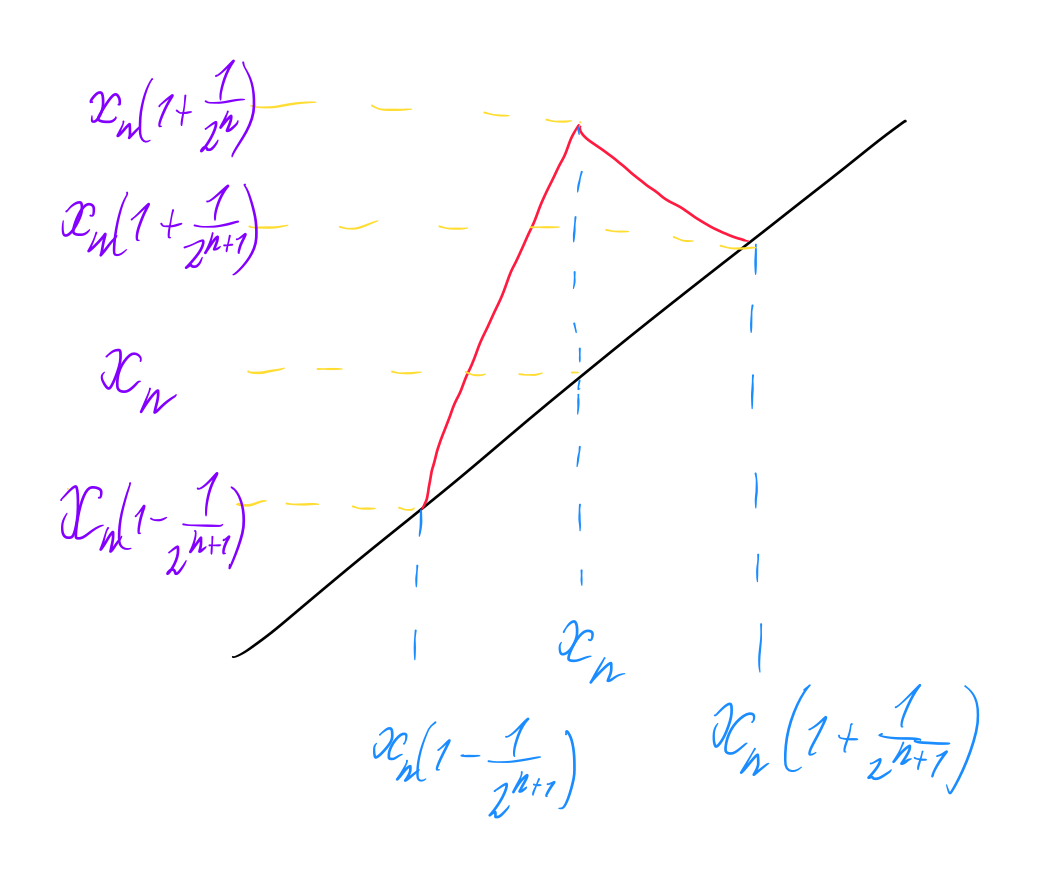
\includegraphics[height=5cm]{MA-practice-solutions-002-02-1.pdf}
            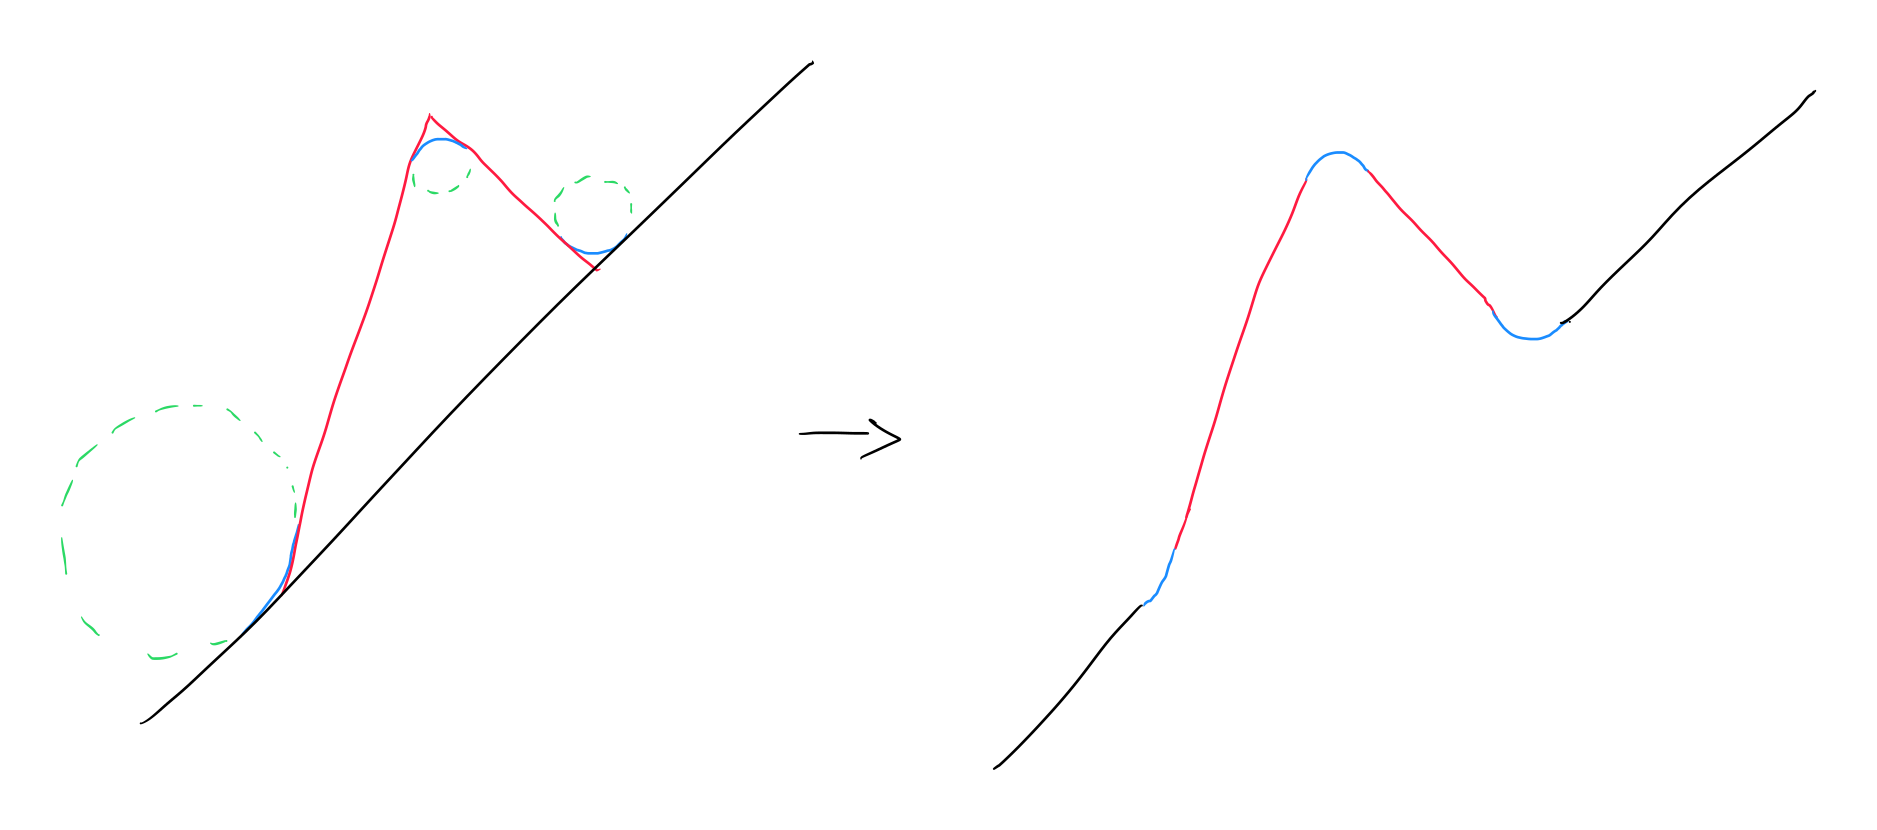
\includegraphics[height=5cm]{MA-practice-solutions-002-02-2.pdf}
        \end{figure}
        Очевидно, что на интервале $(x_n(1-\frac{1}{2^{n+1}}); x_n)$ будет строгое возрастание, а на интервале $(x_n; x_n(1+\frac{1}{2^{n+1}}))$ --- строгое убывание. А это значит, что в любой окрестности нуля не будет никакой монотонности. При этом гладкость нарушается только в точках излома и, может быть, в нуле.
        
        В точках изломах это можно легко исправить, заменив их плавными переходами, например, дугами окружностей (заодно можно сделать их небольшими, чтобы области их действия (интервалы на которых они определены) не пересекались).

        Покажем, что производная в нуле не изменилась. Заметим, что на интервале
        \[(x_n(1-\frac{1}{2^{n+1}}); x_n(1+\frac{1}{2^{n+1}}))\]
        величина $f(x) / x$ всегда не менее $1$, а максимальное отклонение от неё достигается в $x_n$ и равно $1/2^n$. Тогда несложно видеть, что чтобы это отклонение было не больше $1/2^n$ достаточно взять $x_n$-окрестность нуля, так как у всех последующих интервалов (которые как раз расположены в этой окрестности) максимальное отклонение $f(x)/x$ ещё меньше. А значит производная в нуле равна $1$.
    \end{enumproblem}

    \begin{enumproblem}\ 
        \ItemedProblem
        \begin{enumerate}
            \item Давайте докажем существование такой функции для любого не более чем счётного $X$ (для $\QQ$ это будет очевидным следствием). В таком случае есть инъекция $\mu: X \to \NN$. Тогда в качестве $f$ подойдёт $-\mu$. Действительно, пусть дано $x \in X$, тогда множество
                \[Y_x := \{y \in X \mid f(y) \geqslant f(x) \wedge y \neq x\} = \{y \in X \mid \mu(y) < \mu(x)\}\]
                конечно, что значит, что величина $\varepsilon := \min_{y \in Y_x} |y-x|$ абсолютно корректно определена, а в проколотой $\varepsilon$-окрестности $x$ нет точек $Y$, а значит все значения $f$ там же строго меньше, чем в $x$, что и требовалось.
            \item Давайте докажем несуществование такой функции для любого более чем счётного $X$ (для $\RR$ это будет очевидным следствием). Предположим противное, тогда для каждого $x \in X$ есть $\varepsilon_x > 0$, что в проколотой $\varepsilon_x$-окрестности $x$ значения $f$ строго меньше. Заметим, что любые две такие окрестности не должны ``сильно перекрываться'', т.е. для любых двух таких окрестностей верно, что одна из них находится строго с одной стороны относительно центра другой.

                Вспомним, что $|X| > |\NN|$, а тогда существует такая константа $L > 0$, что множество
                \[Y := \{y \in X \mid \varepsilon_y > L\}\]
                более чем счётно. Действительно, иначе
                \[|X| = \left|\bigcup_{n \in \NN} \left\{y \in X \mid \varepsilon_y > \frac{1}{2^n}\right\}\right| \leqslant \sum_{n \in \NN} \left|\left\{y \in X \mid \varepsilon_y > \frac{1}{2^n}\right\}\right| \leqslant \sum_{n \in \NN} |\NN| = |\NN|\]
                откуда $|X| \leqslant |\NN|$, что не верно по условию.

                Заметим, что для любых $y_1, y_2 \in Y$ верно, что $|y_1 - y_2| \geqslant \min(\varepsilon_{y_1}, \varepsilon_{y_2}) > L$. Тогда мы имеем, что для всякого $n \in \ZZ$ верно, что $|Y \cap [nL; (n+1)L)| \leqslant 1$. Значит
                \[|Y| = |Y \cap \RR| = \sum_{n \in \ZZ} |Y \cap [nL; (n+1)L)| \leqslant \sum_{n \in \ZZ} 1 = |\ZZ| = |\NN|\]
                --- противоречие. Значит такой $f$ не существует.
        \end{enumerate}
    \end{enumproblem}

    \begin{enumproblem}\ 
        \ItemedProblem
        \begin{enumerate}
            \item Заметим, что период $\cos(nx)$, в течение которого он принимает все значения из отрезка $[-1; 1]$, равен $2\pi/n$. Это значит, что в замкнутой $2\pi/n$-окрестности любой точки $F_n$ принимает весь отрезок значений $[-1; 1]$. Значит для любого $x \in [0;1]$ можно построить последовательность $\{x_n\}_{n = 0}^\infty$, что $|x-x_n|\leqslant 2\pi/n$, а $F_n(x_n) = -1$. Поэтому если искомая $F$ существует, то
            \[F(x) \leqslant \varliminf_{n \to \infty} F_n(x_n) = \varliminf_{n \to \infty} -1 = -1\]
            Также несложно видеть, что для любой последовательности $\{x_n\}_{n=0}^\infty$, сходящейся к любому $x \in [0; 1]$, верно, что $\{F_n(x_n)\}_{n=0}^\infty \geqslant \{-1\}_{n=0}^\infty$, а значит если искомая $F$ существует, то
            \[F(x) \geqslant \varlimsup_{n \to \infty} F_n(x_n) \geqslant \varliminf_{n \to \infty} -1 = -1\]
            Поэтому единственная подходящая, которая может быть, $F$ --- $F \equiv 1$. Покажем, что эта функция подходит.
            
            Действительно, для любой точки $x$ и любой последовательности $\{x_n\}_{n=0}^\infty$, сходящейся к ней, верно, что
            \[F(x) = -1 = \varliminf_{n \to \infty} -1 \leqslant \varliminf_{n \to \infty} F_n(x_n)\]
            При этом, как мы уже показывали для всякого $x$ есть последовательность $\{x_n\}_{n=0}^\infty$, сходящаяся к $x$, что $\{F_n(x_n)\}_{n=0}^\infty = \{-1\}_{n=0}^\infty$, а значит
            \[F(x) = -1 = \varlimsup_{n \to \infty} -1 = \varlimsup_{n \to \infty} F_n(x_n)\]

            Таким образом гамма-предел равен $F \equiv 1$.

            \item Очевидно, что для всякого $x \in [-1; 1] \setminus \{0\}$, начиная с некоторого $n \in \NN$ в некоторой окрестности $x$ все значения всех функций, начиная с $F_n$, будут равны $0$. Значит гамма-предел $\{F_n\}_{n=0}^\infty$ в любой точке $[-1; 1] \setminus \{0\}$ равен $0$ (оба условия на гамма-предел во всех этих точках верны). Поэтому осталось проверить $x = 0$.
            
            Заметим, что для всякой последовательности $\{a_n\}_{n=0}^\infty$, что $a_n \in [-1;1]$ можно подобрать последовательность $\{x_n\}_{n=0}^\infty$, что $x_n \in [-\pi/n;\pi/n]$ и $F_n(x_n) = a_n$, а в таком случае $\{x_n\}_{n=0}^\infty$ сходится к $0$. Таким образом по аналогии мы имеем, что $F(0) \leqslant -1$ и $F(0) \geqslant -1$, значит $F(0) = -1$. При этому оба условия на гамма-предел выполняются в таком случае: первый выполнен из-за простого условия, что $F(x) \geqslant -1$, а второго из существования последовательности $\{x_n\}_{n=0}^\infty$, сходящейся к $0$, что $F_n(x_n) = -1$ для всякого $n \in \NN \cup \{0\}$.
            
            Таким образом ответ --- $-\mathds{1}_{\{0\}}$.

            \item Заметим, что WLOG можно рассматривать вместо функций с областью значений $[-\infty; +\infty]$ функции с областью определением $[-1; 1]$. Действительно, пусть $\tau: [-\infty; +\infty] \to [-1;1]$ --- монотонная биекция (например, $2\arctan/\pi$, доопределённая в $\pm\infty$ как $\pm 1$ соответственно), тогда условия на то, чтобы $F$ являлся гамма-пределом $\{F_n\}_{n=0}^\infty$, равносильны условиям на то, чтобы $F\circ \mu^{-1}$ являлся гамма-пределом $\{F_n \circ \mu^{-1}\}_{n=0}^\infty$. Поэтому теперь будем думать только о функциях $[0; 1] \to [-1; 1]$.

            Сначала покажем, что предел $\lim_{n \to \infty} \inf(F_n)$ определён. Предположим противное. Очевидно, у последовательности $\{\inf(F_N)\}_{n=0}^\infty$ (как и любой другой ограниченной последовательности) есть предельные точки, частными случаями которых являются верхний и нижний предел этой же последовательности (они так же определены). Пусть $a$ --- нижний предел. То, что он не является пределом последовательности значит, что есть $\varepsilon > 0$, что есть бесконечно много членов последовательности, неменьших $a + \varepsilon$. Мы знаем, что для некоторой строго возрастающей последовательности $\{i_n\}_{n=0}^\infty$ натуральных чисел верно, что $\{\inf(F_{i_n})\}_{n=0}^\infty \to a$. Значит мы можем взять последовательность $\{t_n\}_{n=0}^\infty$ точек, что
            \[F_{i_n}(t_n) - \inf(F_{i_n}) < 1/2^n\]
            В таком случае можно взять сходящуюся подпоследовательность $\{s_n\}_{n=0}^\infty$ последовательности $\{t_n\}_{n=0}^\infty$ и соответствующую ей подпоследовательность $\{j_n\}_{n=0}^\infty$ последовательности $\{i_n\}_{n=0}^\infty$. Пусть $\lim \{s_n\}_{n=0}^\infty = S$. Тогда можно рассмотреть последовательность $\{x_n\}_{n=0}^\infty$, что для всякого $k \in \NN \cup \{0\}$ $x_{j_k} := s_k$, а остальные члены определены случайным образом так, чтобы $\{x_n\}_{n=0}^\infty$ сошлась к $S$. В таком случае
            \[\varliminf_{n \to \infty} F_n(x_n) = a\]
            Так как подпоследовательность $\{F_{j_k}(s_k)\}_{k=0}^\infty$ уже сходится к $a$, а с другой стороны $a$ --- нижний предел $\{\inf(F_n)\}_{n=0}^\infty$, поэтому очевидно, что нижний предел не может быть ниже $a$. При этом для любой абсолютно последовательности $\{y_n\}_{n=0}^\infty$, сходящейся к $S$, после любого момента найдётся такое $k$, что $\inf(F_k) \geqslant a + \varepsilon$, и т.е. $F_k(x_k) \geqslant a + \varepsilon$, поэтому верхний предел любой такой последовательности не менее $a + \varepsilon$. А в таком случае мы имеем, что
            \[a + \varepsilon \leqslant F(S) \leqslant a\]
            --- противоречие. Значит предел инфимумов определён.

            Теперь покажем, что предел равен $\inf(F)$. Для начала покажем, что он не более чем $\inf(F)$. Действительно, для любого $\varepsilon > 0$ найдётся точка $x \in [0; 1]$, что $F(x) - \inf(F) < \varepsilon/2$. Для неё по определению гамма-предела есть последовательность $\{x_n\}_{n=0}^\infty$, что $\lim \{x_n\}_{n=0}^\infty = x$, а $\varlimsup \{F_n(x_n)\}_{n=0}^\infty \leqslant F(x)$. Тогда мы имеем, что есть такое $k$, что $F_k(x_k) < F(x) + \varepsilon/2$, а тогда
            \[\inf(F_k) \leqslant F_k(x_k) < F(x) + \frac{\varepsilon}{2} < \inf(F) + \varepsilon\]
            Значит $\lim \{\inf(F_n)\}_{n=0}^\infty \leqslant \inf(F)$.

            Теперь покажем, что $\lim \{\inf(F_n)\}_{n=0}^\infty \geqslant \inf(F)$. Построим последовательность $\{x_n\}_{n=0}^\infty$, что $F_n(x_n) - \inf(F_n) < 1/2^n$. Затем сотрём в этой последовательности некоторые члены, чтобы получившаяся подпоследовательность сходилась, а на место стёртых поставим случайные точки, так чтобы вся последовательность сошлась; получим $\{y_n\}_{n=0}^\infty$ Тогда $\lim \{\inf(F_n)\}_{n=0}^\infty$ является предельной точкой $\{F_n(y_n)\}_{n=0}^\infty$. Поэтому
            \[\inf(F) \leqslant F\left(\lim \{y_n\}_{n=0}^\infty\right) \leqslant \varliminf \{F_n(y_n)\}_{n=0}^\infty \leqslant \lim \{\inf(F_n)\}_{n=0}^\infty\]
            
            Таким образом $\lim_{n \to \infty} \inf(F_n)$ определён и равен $\inf(F)$.
        \end{enumerate}
    \end{enumproblem}

    \begin{enumproblem}
        Рассмотрим $g: [0; +\infty) \to [0; +\infty), x \mapsto -\ln(f(\exp(x)))$. Заметим, что $g$ по своей сути является той же $f$, но ``в других координатах''. Также дифференцируемость $f$ в единице равносильна дифференцируемости $g$ в нуле. При этом мы получили от $f$, что
        \begin{itemize}
            \item $g(0) = 0$;
            \item $g(x + y) \geqslant g(x) + g(y)$.
        \end{itemize}
        Поэтому докажем, что $g$ дифференцируема в нуле. Для этого также рассмотрим $h: (0; +\infty) \to [0; +\infty), x \mapsto g(x)/x$. Таким образом нужно показать, что $\lim_{x \to 0^+} h(x)$ определён.

        Заметим, что
        \begin{itemize}
            \item $g$ монотонно неубывает, так как если $x > y$, то $g(x) \geqslant g(y) + g(x-y) \geqslant g(y)$;
            \item $\forall n \in \NN \setminus \{0\}$ и $x \geqslant 0$ верно, что $g(nx) \geqslant ng(x)$, а следовательно $g(x/n) \leqslant g(x)/n$.
        \end{itemize}
        Тогда покажем, что для всякого $x > 0$
        \[\varlimsup_{t \to 0^+} h(t) \leqslant h(x)\]
        Рассмотрим $t \in [x/(n+1); x/n]$ для всякого $n \in \NN\setminus\{0\}$. Заметим, что
        \[h(t) = \frac{g(t)}{t} \leqslant \frac{g(x/n)}{x/(n+1)} \leqslant \frac{g(x)/n}{x/(n+1)} = h(x) \cdot \frac{n+1}{n}\]
        Следовательно для всякого $t \in (0; x/n)$ верно, что $h(t) \leqslant h(x) \cdot (n+1)/n$, а тогда
        \[\varlimsup_{t \to 0^+} h(t) \leqslant \lim_{n \to \infty} h(x) \cdot \frac{n+1}{n} = h(x)\]
        Теперь рассмотрим последовательность $\{x_n\}_{n=0}^\infty$, сходящуюся к $0$, что
        \[\lim_{n \to \infty} h(x_n) = \varliminf_{t \to 0^+} h(t)\]
        Тогда заметим, что для всякого $n \in \NN \cup \{0\}$
        \[\varlimsup_{t \to 0^+} h(t) \leqslant h(x_n)\]
        а следовательно
        \[\varlimsup_{t \to 0^+} h(t) \leqslant \lim_{n \to \infty} h(x_n) = \varliminf_{t \to 0^+} h(t)\]
        Следовательно верхний и нижний пределы $h(t)$ при $t \to 0^+$ совпали, а значит и обычный предел определён.
    \end{enumproblem}

    \begin{enumproblem}
        TBP
    \end{enumproblem}

    \begin{enumproblem}
        TBP
    \end{enumproblem}

    \begin{enumproblem}
        Будем считать, что $f$ монотонно не убывает; иначе рассмотрим $-f$ вместо $f$.
        \ItemedProblem
        \begin{enumerate}
            \item Заметим, что для $x \in [1/(n+1); 1/n]$ верно, что
            \begin{multline*}
                \frac{f(1/(n+1)) - f(0)}{1/(n+1)} \cdot \frac{n}{n+1} = \frac{f(1/(n+1)) - f(0)}{1/n}\\
                \leqslant \frac{f(x) - f(0)}{x} \leqslant\\
                \frac{f(1/n) - f(0)}{1/(n+1)} = \frac{f(1/n) - f(0)}{1/n} \cdot \frac{n+1}{n}
            \end{multline*}
            Поэтому очевидно, что
            \begin{multline*}
                \lim_{\substack{x \to 0^+\\x \in A}} \frac{f(x) - f(0)}{x} = \lim_{n \to \infty} \frac{f(1/(n+1)) - f(0)}{1/(n+1)} \cdot \frac{n}{n+1}\\
                \leqslant \lim_{x \to 0^+} \frac{f(x) - f(0)}{x} \leqslant\\
                \lim_{n \to \infty} \frac{f(1/n) - f(0)}{1/n} \cdot \frac{n+1}{n} = \lim_{\substack{x \to 0^+\\x \in A}} \frac{f(x) - f(0)}{x}
            \end{multline*}
            то есть
            \[\lim_{x \to 0^+} \frac{f(x) - f(0)}{x} = \lim_{\substack{x \to 0^+\\x \in A}} \frac{f(x) - f(0)}{x}\]
            Аналогично
            \[\lim_{x \to 0^+} \frac{f(x) - f(0)}{x} = \lim_{\substack{x \to 0^-\\x \in A}} \frac{f(x) - f(0)}{x}\]
            Это значит, что $f$ дифференцируема в нуле.

            \item Определим
            \[
                f: \RR \to \RR, x \mapsto
                \begin{cases}
                    0& \text{если $x = 0$}\\
                    \sign(x) \cdot 2^{\lceil \log_2|x| \rceil}& \text{иначе}
                \end{cases}
            \]
            Пусть $|x| \in (2^n; 2^{n+1}]$, где $n \in \ZZ$. Тогда $\log_2|x| = n+1$, а значит $f(x) = \sign(x) \cdot 2^{n+1}$. Следовательно
            \[\frac{f(x) - f(0)}{x} = \frac{2^{n+1}}{|x|} \in \left[\frac{2^{n+1}}{2^{n+1}}; \frac{2^{n+1}}{2^n}\right) = [1; 2)\]
            При этом все значения полуинтервала достигаются. А значит в любой окрестности $0$ выражение
            \[\frac{f(x) - f(0)}{x}\]
            болтается по полуинтервалу $[1; 2)$, поэтому $f$ недифференцируема в нуле.
            
            Несмотря на это для всякого $n \in \ZZ$ мы имеем, что $f(\pm 2^n) = \pm 2^n$, а значит
            \[\lim_{\substack{x \to 0\\x\in A}} \frac{f(x) - f(0)}{x} = \lim_{\substack{x \to 0\\x\in A}} 1 = 1\]

            Поэтому для данного $A$ утверждение неверно.
        \end{enumerate}
    \end{enumproblem}

    \begin{enumproblem}\ 
        \begin{enumerate}
            \item Заметим, что если $x \not\equiv 0 \pmod{2\pi}$
            \begin{gather*}
                \sum_{k = 1}^n \sin(kx) = \sum_{k = 0}^n \Im(e^{ikx}) = \Im\left(\sum_{k = 0}^n e^{ikx}\right) = \Im\left(\frac{e^{i(n+1)x} - 1}{e^{ix} - 1}\right) \leqslant \frac{|e^{i(n+1)x} - 1|}{|e^{ix} - 1|} \leqslant \frac{2}{|e^{ix} - 1|}
            \end{gather*}
            Поэтому префиксные суммы последовательности $\{\sin(nx)\}_{n=1}^\infty$ ограничены; при этом последовательность
            \[\left\{\frac{1}{n^\alpha}\right\}_{n=1}^\infty\]
            сходится монотонно сверху к нулю. Таким образом по принципу Дирихле ряд $\sum_{n=1}^\infty \frac{\sin(nx)}{n^\alpha}$ сходится.

            \item Заметим, что для всякого $n \in \NN \setminus \{0\}$
            \[\sum_{k=1}^{2n} \frac{\sin(k \frac{\pi}{4n})}{k^\alpha} \geqslant \sum_{k=n+1}^{2n} \frac{\sin(k \frac{\pi}{4n})}{k} \geqslant \sum_{k=n+1}^{2n} \frac{\sin(\pi/4)}{k} \geqslant \frac{1}{\sqrt{2}} \sum_{k=n+1}^{2n} \frac{1}{2n} \geqslant \frac{1}{2\sqrt{2}}\]
            Заметим, что это префикс длины $2n$ в точке $x = \frac{\pi}{4n}$.

            Если ряд равномерно сходится при $x \in [-1; 1]$, то предельная $f(x)$ будет непрерывна. Значит для всякого $\varepsilon > 0$ есть $\delta > 0$, что в $\delta$-окрестности $0$ значения $|f(x)|$ будут менее $\varepsilon/2$. При этом по равномерной сходимости будет такое $N \in \NN \setminus \{0\}$, что все префиксные суммы начиная с $S_N$ будут находится в $\varepsilon/2$-окрестностях соответствующих значений $f$. Поэтому в $\delta$-окрестности все префиксные суммы начиная с $S_N$ будут менее $\varepsilon$. С другой стороны мы знаем, что для всякого $n \in \NN \setminus \{0\}$ будет $S_2n(\pi/4n) \geqslant 1/2\sqrt{2}$, т.е. в любой окрестности $0$ после любого момента будет префиксная сумма, которая не менее $1/2\sqrt{2}$, а значит она для $\varepsilon = 1/4\sqrt{2}$ утверждение равномерной сходимости неверно.

            \item Заметим, что если бы ряд сходился равномерно по $\alpha$, то для всякого $\varepsilon > 0$ было бы $N \in \NN \setminus \{0\}$, что все префиксные суммы после $S_N$ были бы в $\varepsilon$-окрестности предельного значения. При этом заметим, что $\{\sin(nx)\}_{n=1}^\infty$ принимает значения из любой окрестности супремума бесконечно много раз. Пусть супремум этой последовательности равен $C > 0$, тогда для всякого $N \in \NN \setminus \{0\}$ можно подобрать $n > N$, что $\sin(nx) > C/\sqrt{2}$; также можно подобрать $\alpha > 0$, что $n^\alpha < \sqrt{2}$, следовательно $\sin(nx)/n^\alpha > C/2$, поэтому $|S_n - S_{n-1}| > C/2$. Таким образом для $\varepsilon = C/4$ нет такого $N$, что все префиксные суммы больше не будут разбросаны вне $\varepsilon$-окрестностей предельных значений. 
        \end{enumerate}
    \end{enumproblem}

    \section*{Рейтинговые задачи}

    \begin{enumproblem}
        TBP
    \end{enumproblem}

    \begin{enumproblem}
        TBP
    \end{enumproblem}

    \begin{enumproblem}
        TBP
    \end{enumproblem}

    \begin{enumproblem}
        TBP
    \end{enumproblem}

    \begin{enumproblem}
        TBP
    \end{enumproblem}

    \begin{enumproblem}
        TBP
    \end{enumproblem}

    \begin{enumproblem}
        TBP
    \end{enumproblem}
    
\end{document}